
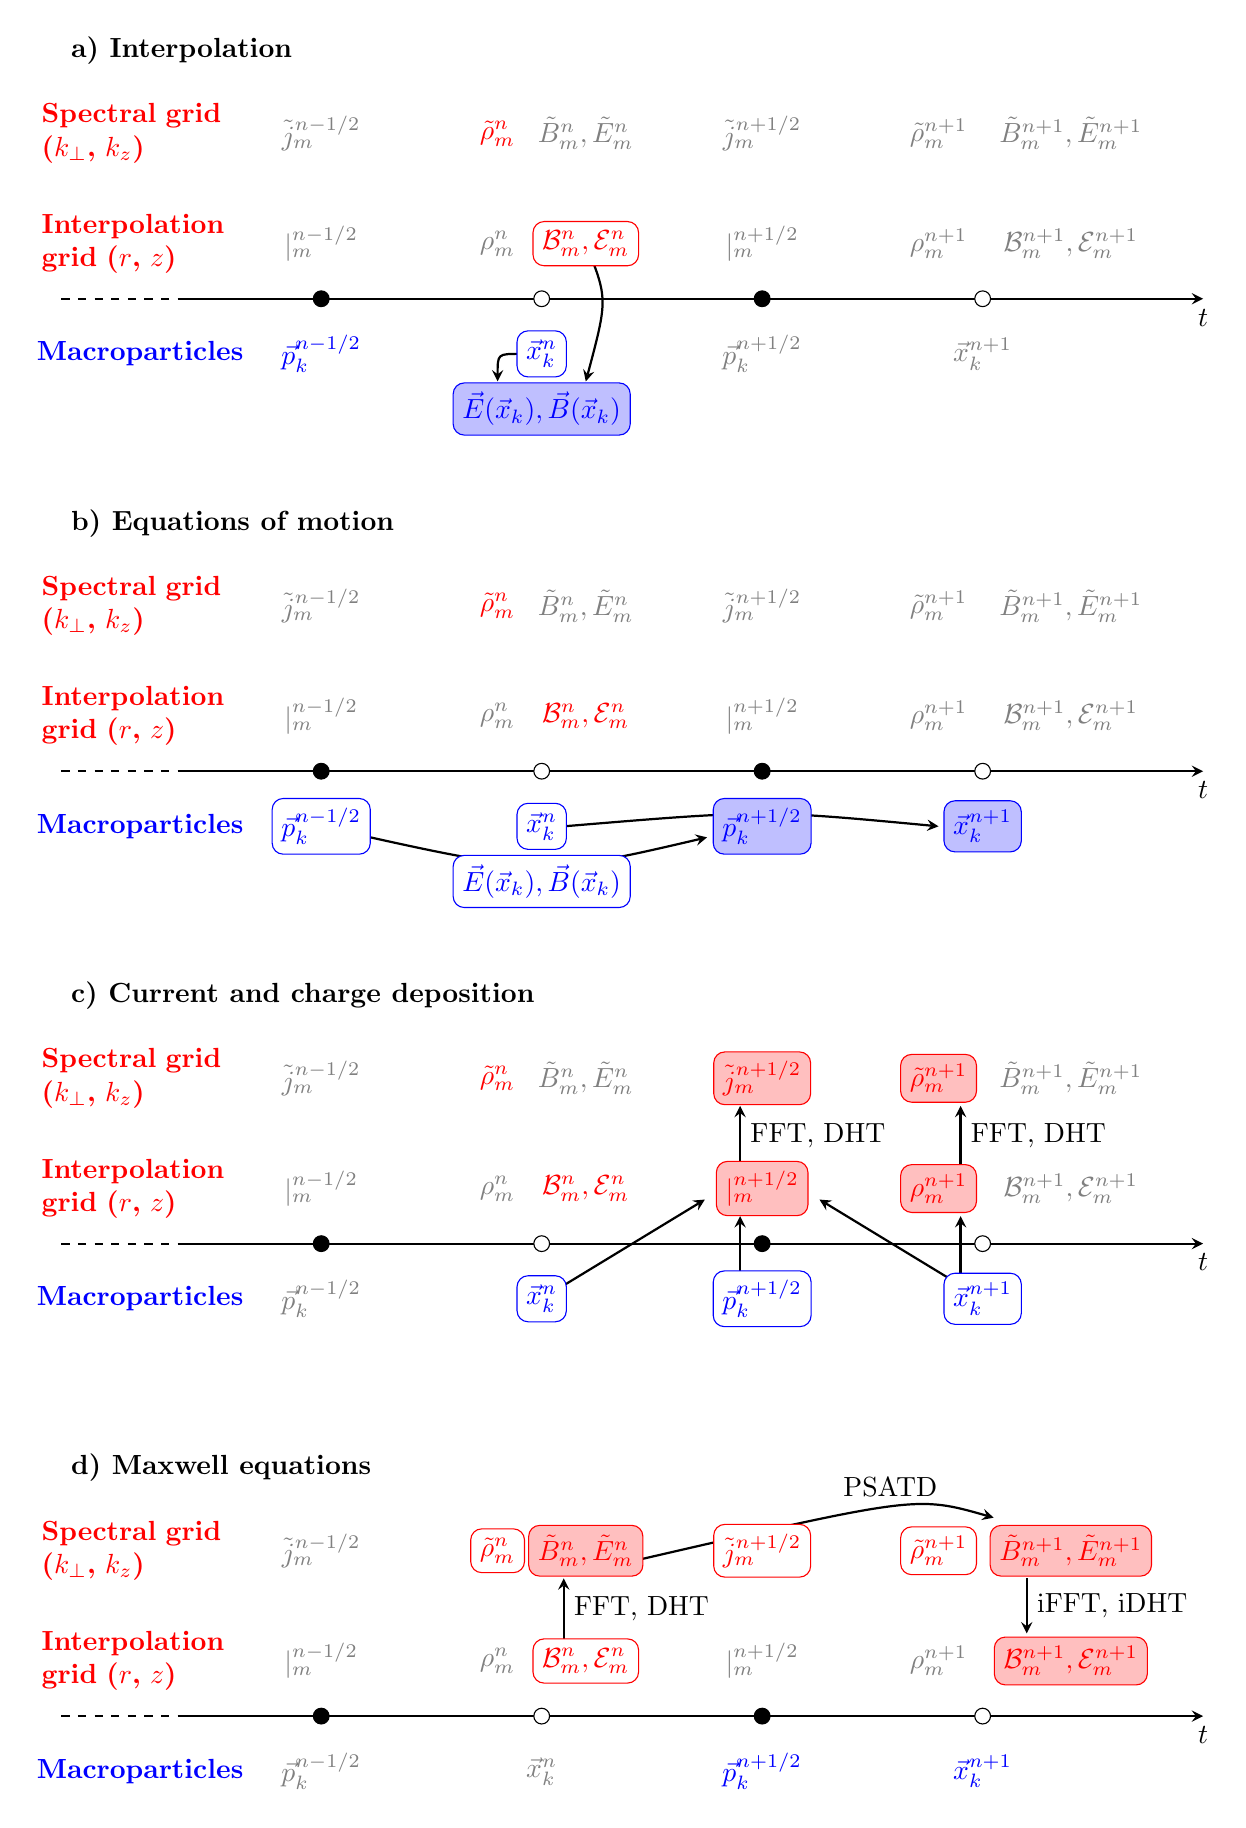
\begin{tikzpicture}
\def \Dt{2.8}
\def \yspac{0.7}

\begin{scope}[yshift=0cm]

\draw (-0.5,4.5*\yspac) node[anchor=west]{\textbf{a) Interpolation}};

% Axes
\draw[thick,->,>=stealth] (1,0) -- (5*\Dt,0) node[below]{$t$};
\draw[thick,dashed] (-0.5,0) -- (1,0);
% Labels
\draw (0.5,3*\yspac) node[red,text width=2.5cm]{\textbf{Spectral grid ($k_\perp$, $k_z$)}};
\draw (0.5,\yspac) node[red,text width=2.5cm]{\textbf{Interpolation grid ($r$, $z$)}};
\draw (0.5,-\yspac) node[blue]{\textbf{Macroparticles}};
% Timesteps
\foreach \n in {1,3} 
\draw[fill=black] (\n*\Dt,0) circle(0.1);
\foreach \n in {2,4} 
\draw[fill=white] (\n*\Dt,0) circle(0.1);
% Arrows
%\draw[->,>=stealth,thick] (3*\Dt,\yspac) -- (2.5*\Dt,-0.25);
%\draw[->,>=stealth,thick] (1.85*\Dt,\yspac) -- (1.85*\Dt,-0.25);
\draw[->,>=stealth,thick] (2.2*\Dt,\yspac) .. controls (2.3*\Dt,0) .. (2.2*\Dt,-1.5*\yspac);
\draw[->,>=stealth,thick] (1.9*\Dt,-1*\yspac) .. controls (1.8*\Dt,-1*\yspac) .. (1.8*\Dt,-1.5*\yspac);
% Fields
% -- n-1/2
\draw (\Dt,3*\yspac) node[gray,fill=white,draw=white,rounded corners]{$ \tilde{j}^{n-1/2}_m$};
\draw (\Dt,1*\yspac) node[gray,fill=white,draw=white,rounded corners]{$ \mathcal{j}^{n-1/2}_m$};
\draw (\Dt,-\yspac) node[blue]{$\vec{p}_k^{n-1/2}$};
% -- n
\draw (1.8*\Dt,3*\yspac) node[red,fill=white,draw=white,rounded corners]{$\tilde{\rho}^n_m$};
\draw (2.2*\Dt,3*\yspac) node[gray,fill=white,draw=white,rounded corners]{$  \tilde{B}^{n}_m, \tilde{E}^{n}_m$};
\draw (1.8*\Dt,\yspac) node[gray,fill=white,draw=white,rounded corners]{$\mathcal{\rho}^n_m$};
\draw (2.2*\Dt,\yspac) node[red,fill=white,draw=red,rounded corners]{$\mathcal{B}^{n}_m, \mathcal{E}^{n}_m$};
\draw (2*\Dt,-\yspac) node[blue,fill=white,draw=blue,rounded corners]{$\vec{x}_k^{n}$};
\draw (2*\Dt,-2*\yspac) node[blue,fill=white!75!blue,draw=blue,rounded corners]{$\vec{E}(\vec{x}_k), \vec{B}(\vec{x}_k)$};
% -- n+1/2
\draw (3*\Dt,3*\yspac) node[gray,fill=white,draw=white,rounded corners]{$ \tilde{j}^{n+1/2}_m$};
\draw (3*\Dt,1*\yspac) node[gray,fill=white,draw=white,rounded corners]{$ \mathcal{j}^{n+1/2}_m$};
\draw (3*\Dt,-\yspac) node[gray]{$\vec{p}_k^{n+1/2}$};
% -- n+1
\draw (3.8*\Dt,3*\yspac) node[gray,fill=white,draw=white,rounded corners]{$\tilde{\rho}^{n+1}_m$};
\draw (4.4*\Dt,3*\yspac) node[gray,fill=white,draw=white,rounded corners]{$  \tilde{B}^{n+1}_m, \tilde{E}^{n+1}_m$};
\draw (3.8*\Dt,\yspac) node[gray,fill=white,draw=white,rounded corners]{$\mathcal{\rho}^{n+1}_m$};
\draw (4.4*\Dt,\yspac) node[gray,fill=white,draw=white,rounded corners]{$\mathcal{B}^{n+1}_m, \mathcal{E}^{n+1}_m$};
\draw (4*\Dt,-\yspac) node[gray]{$\vec{x}_k^{n+1}$};

\end{scope}

\begin{scope}[yshift=-6cm]

\draw (-0.5, 4.5*\yspac) node[anchor=west]{\textbf{b) Equations of motion}};
% Axes
\draw[thick,->,>=stealth] (1,0) -- (5*\Dt,0) node[below]{$t$};
\draw[thick,dashed] (-0.5,0) -- (1,0);
% Labels
\draw (0.5,3*\yspac) node[red,text width=2.5cm]{\textbf{Spectral grid ($k_\perp$, $k_z$)}};
\draw (0.5,\yspac) node[red,text width=2.5cm]{\textbf{Interpolation grid ($r$, $z$)}};
\draw (0.5,-\yspac) node[blue]{\textbf{Macroparticles}};
% Timesteps
\foreach \n in {1,3} 
\draw[fill=black] (\n*\Dt,0) circle(0.1);
\foreach \n in {2,4} 
\draw[fill=white] (\n*\Dt,0) circle(0.1);
% Arrows
%\draw[->,>=stealth,thick] (\Dt,\yspac) -- (1.5*\Dt,-0.25);
%\draw[->,>=stealth,thick] (3*\Dt,\yspac) -- (2.5*\Dt,-0.25);
%\draw[->,>=stealth,thick] (1.85*\Dt,\yspac) -- (1.85*\Dt,-0.25);
\draw[->,>=stealth,thick] (1*\Dt,-\yspac) .. controls (2*\Dt,-1.9*\yspac) .. (2.75*\Dt,-1.2*\yspac);
\draw[->,>=stealth,thick] (2.1*\Dt,-1*\yspac) .. controls (3*\Dt,-0.7*\yspac) .. (3.8*\Dt,-1.*\yspac);
% Fields
% -- n-1/2
\draw (\Dt,3*\yspac) node[gray,fill=white,draw=white,rounded corners]{$ \tilde{j}^{n-1/2}_m$};
\draw (\Dt,1*\yspac) node[gray,fill=white,draw=white,rounded corners]{$ \mathcal{j}^{n-1/2}_m$};
\draw (\Dt,-\yspac) node[blue,fill=white,draw=blue,rounded corners]{$\vec{p}_k^{n-1/2}$};
% -- n
\draw (1.8*\Dt,3*\yspac) node[red,fill=white,draw=white,rounded corners]{$\tilde{\rho}^n_m$};
\draw (2.2*\Dt,3*\yspac) node[gray,fill=white,draw=white,rounded corners]{$  \tilde{B}^{n}_m, \tilde{E}^{n}_m$};
\draw (1.8*\Dt,\yspac) node[gray,fill=white,draw=white,rounded corners]{$\mathcal{\rho}^n_m$};
\draw (2.2*\Dt,\yspac) node[red,fill=white,draw=white,rounded corners]{$\mathcal{B}^n_m, \mathcal{E}^{n}_m$};
\draw (2*\Dt,-\yspac) node[blue,fill=white,draw=blue,rounded corners]{$\vec{x}_k^{n}$};
\draw (2*\Dt,-2*\yspac) node[blue,fill=white,draw=blue,rounded corners]{$\vec{E}(\vec{x}_k), \vec{B}(\vec{x}_k)$};
% -- n+1/2
\draw (3*\Dt,3*\yspac) node[gray,fill=white,draw=white,rounded corners]{$ \tilde{j}^{n+1/2}_m$};
\draw (3*\Dt,1*\yspac) node[gray,fill=white,draw=white,rounded corners]{$ \mathcal{j}^{n+1/2}_m$};
\draw (3*\Dt,-\yspac) node[blue,fill=white!75!blue,draw=blue,rounded corners]{$\vec{p}_k^{n+1/2}$};
% -- n+1
\draw (3.8*\Dt,3*\yspac) node[gray,fill=white,draw=white,rounded corners]{$\tilde{\rho}^{n+1}_m$};
\draw (4.4*\Dt,3*\yspac) node[gray,fill=white,draw=white,rounded corners]{$  \tilde{B}^{n+1}_m, \tilde{E}^{n+1}_m$};
\draw (3.8*\Dt,\yspac) node[gray,fill=white,draw=white,rounded corners]{$\mathcal{\rho}^{n+1}_m$};
\draw (4.4*\Dt,\yspac) node[gray,fill=white,draw=white,rounded corners]{$\mathcal{B}^{n+1}_m, \mathcal{E}^{n+1}_m$};
\draw (4*\Dt,-\yspac) node[blue,fill=white!75!blue,draw=blue,rounded corners]{$\vec{x}_k^{n+1}$};

\end{scope}

\begin{scope}[yshift=-12cm]

\draw (-0.5,4.5*\yspac) node[anchor=west]{\textbf{c) Current and charge deposition}};

% Axes
\draw[thick,->,>=stealth] (1,0) -- (5*\Dt,0) node[below]{$t$};
\draw[thick,dashed] (-0.5,0) -- (1,0);
% Labels
\draw (0.5,3*\yspac) node[red,text width=2.5cm]{\textbf{Spectral grid ($k_\perp$, $k_z$)}};
\draw (0.5,\yspac) node[red,text width=2.5cm]{\textbf{Interpolation grid ($r$, $z$)}};
\draw (0.5,-\yspac) node[blue]{\textbf{Macroparticles}};
% Timesteps
\foreach \n in {1,3} 
\draw[fill=black] (\n*\Dt,0) circle(0.1);
\foreach \n in {2,4} 
\draw[fill=white] (\n*\Dt,0) circle(0.1);
% Arrows
\draw[->,>=stealth,thick] (2*\Dt,-\yspac) -- (2.74*\Dt,0.8*\yspac);
\draw[->,>=stealth,thick] (2.9*\Dt,-\yspac) -- (2.9*\Dt,0.5*\yspac);
\draw[->,>=stealth,thick] (2.9*\Dt,1.4*\yspac) -- node[anchor=west]{FFT, DHT}(2.9*\Dt,2.5*\yspac);
\draw[->,>=stealth,thick] (4*\Dt,-\yspac) -- (3.26*\Dt,0.8*\yspac);
\draw[->,>=stealth,thick] (3.9*\Dt,-\yspac) -- (3.9*\Dt,0.5*\yspac);
\draw[->,>=stealth,thick] (3.9*\Dt,1.4*\yspac) -- node[anchor=west]{FFT, DHT}(3.9*\Dt,2.5*\yspac);
%\draw[->,>=stealth,thick] (3*\Dt,\yspac) -- (2.5*\Dt,-0.25);
%\draw[->,>=stealth,thick] (1.85*\Dt,\yspac) -- (1.85*\Dt,-0.25);
%\draw[->,>=stealth,thick] (1*\Dt,-\yspac) .. controls (2*\Dt,-1.9*\yspac) .. (2.75*\Dt,-1.2*\yspac);
%\draw[->,>=stealth,thick] (2.1*\Dt,-1*\yspac) .. controls (3*\Dt,-0.7*\yspac) .. (3.8*\Dt,-1.*\yspac);
% Fields
% -- n-1/2
\draw (\Dt,3*\yspac) node[gray,fill=white,draw=white,rounded corners]{$ \tilde{j}^{n-1/2}_m$};
\draw (\Dt,1*\yspac) node[gray,fill=white,draw=white,rounded corners]{$ \mathcal{j}^{n-1/2}_m$};
\draw (\Dt,-\yspac) node[gray,fill=white,draw=white,rounded corners]{$\vec{p}_k^{n-1/2}$};
% -- n
\draw (1.8*\Dt,3*\yspac) node[red,fill=white,draw=white,rounded corners]{$\tilde{\rho}^n_m$};
\draw (2.2*\Dt,3*\yspac) node[gray,fill=white,draw=white,rounded corners]{$  \tilde{B}^{n}_m, \tilde{E}^{n}_m$};
\draw (1.8*\Dt,\yspac) node[gray,fill=white,draw=white,rounded corners]{$\mathcal{\rho}^n_m$};
\draw (2.2*\Dt,\yspac) node[red,fill=white,draw=white,rounded corners]{$\mathcal{B}^n_m, \mathcal{E}^{n}_m$};
\draw (2*\Dt,-\yspac) node[blue,fill=white,draw=blue,rounded corners]{$\vec{x}_k^{n}$};
% -- n+1/2
\draw (3*\Dt,3*\yspac) node[red,fill=white!75!red,draw=red,rounded corners]{$ \tilde{j}^{n+1/2}_m$};
\draw (3*\Dt,1*\yspac) node[red,fill=white!75!red,draw=red,rounded corners]{$ \mathcal{j}^{n+1/2}_m$};
\draw (3*\Dt,-\yspac) node[blue,fill=white,draw=blue,rounded corners]{$\vec{p}_k^{n+1/2}$};
% -- n+1
\draw (3.8*\Dt,3*\yspac) node[red,fill=white!75!red,draw=red,rounded corners]{$\tilde{\rho}^{n+1}_m$};
\draw (4.4*\Dt,3*\yspac) node[gray,fill=white,draw=white,rounded corners]{$  \tilde{B}^{n+1}_m, \tilde{E}^{n+1}_m$};
\draw (3.8*\Dt,\yspac) node[red,fill=white!75!red,draw=red,rounded corners]{$\mathcal{\rho}^{n+1}_m$};
\draw (4.4*\Dt,\yspac) node[gray,fill=white,draw=white,rounded corners]{$\mathcal{B}^{n+1}_m, \mathcal{E}^{n+1}_m$};
\draw (4*\Dt,-\yspac) node[blue,fill=white,draw=blue,rounded corners]{$\vec{x}_k^{n+1}$};

\end{scope}

\begin{scope}[yshift=-18cm]

\draw (-0.5,4.5*\yspac) node[anchor=west]{\textbf{d) Maxwell equations}};

% Axes
\draw[thick,->,>=stealth] (1,0) -- (5*\Dt,0) node[below]{$t$};
\draw[thick,dashed] (-0.5,0) -- (1,0);
% Labels
\draw (0.5,3*\yspac) node[red,text width=2.5cm]{\textbf{Spectral grid ($k_\perp$, $k_z$)}};
\draw (0.5,\yspac) node[red,text width=2.5cm]{\textbf{Interpolation grid ($r$, $z$)}};
\draw (0.5,-\yspac) node[blue]{\textbf{Macroparticles}};
% Timesteps
\foreach \n in {1,3} 
\draw[fill=black] (\n*\Dt,0) circle(0.1);
\foreach \n in {2,4} 
\draw[fill=white] (\n*\Dt,0) circle(0.1);
% Arrows
%\draw[->,>=stealth,thick] (2*\Dt,-\yspac) -- (2.74*\Dt,0.8*\yspac);
%\draw[->,>=stealth,thick] (2.9*\Dt,-\yspac) -- (2.9*\Dt,0.5*\yspac);
\draw[->,>=stealth,thick] (2.1*\Dt,1.4*\yspac) -- node[anchor=west]{FFT, DHT}(2.1*\Dt,2.5*\yspac);
%\draw[->,>=stealth,thick] (4*\Dt,-\yspac) -- (3.26*\Dt,0.8*\yspac);
%\draw[->,>=stealth,thick] (3.9*\Dt,-\yspac) -- (3.9*\Dt,0.5*\yspac);
\draw[<-,>=stealth,thick] (4.2*\Dt,1.5*\yspac) -- node[anchor=west]{iFFT, iDHT}(4.2*\Dt,2.5*\yspac);
%\draw[->,>=stealth,thick] (3*\Dt,\yspac) -- (2.5*\Dt,-0.25);
%\draw[->,>=stealth,thick] (1.85*\Dt,\yspac) -- (1.85*\Dt,-0.25);
%\draw[->,>=stealth,thick] (1*\Dt,-\yspac) .. controls (2*\Dt,-1.9*\yspac) .. (2.75*\Dt,-1.2*\yspac);
\draw[->,>=stealth,thick] (2.4*\Dt,2.8*\yspac) .. controls (3.7*\Dt,4*\yspac) .. node[above]{PSATD} (4.05*\Dt,3.6*\yspac);
% Fields
% -- n-1/2
\draw (\Dt,3*\yspac) node[gray,fill=white,draw=white,rounded corners]{$ \tilde{j}^{n-1/2}_m$};
\draw (\Dt,1*\yspac) node[gray,fill=white,draw=white,rounded corners]{$ \mathcal{j}^{n-1/2}_m$};
\draw (\Dt,-\yspac) node[gray,fill=white,draw=white,rounded corners]{$\vec{p}_k^{n-1/2}$};
% -- n
\draw (1.8*\Dt,3*\yspac) node[red,fill=white,draw=red,rounded corners]{$\tilde{\rho}^n_m$};
\draw (2.2*\Dt,3*\yspac) node[red,fill=white!75!red,draw=red,rounded corners]{$  \tilde{B}^{n}_m, \tilde{E}^{n}_m$};
\draw (1.8*\Dt,\yspac) node[gray,fill=white,draw=white,rounded corners]{$\mathcal{\rho}^n_m$};
\draw (2.2*\Dt,\yspac) node[red,fill=white,draw=red,rounded corners]{$\mathcal{B}^n_m, \mathcal{E}^{n}_m$};
\draw (2*\Dt,-\yspac) node[gray]{$\vec{x}_k^{n}$};
% -- n+1/2
\draw (3*\Dt,3*\yspac) node[red,fill=white,draw=red,rounded corners]{$ \tilde{j}^{n+1/2}_m$};
\draw (3*\Dt,1*\yspac) node[gray,fill=white,draw=white,rounded corners]{$ \mathcal{j}^{n+1/2}_m$};
\draw (3*\Dt,-\yspac) node[blue]{$\vec{p}_k^{n+1/2}$};
% -- n+1
\draw (3.8*\Dt,3*\yspac) node[red,fill=white,draw=red,rounded corners]{$\tilde{\rho}^{n+1}_m$};
\draw (4.4*\Dt,3*\yspac) node[red,fill=white!75!red,draw=red,rounded corners]{$  \tilde{B}^{n+1}_m, \tilde{E}^{n+1}_m$};
\draw (3.8*\Dt,\yspac) node[gray,fill=white,draw=white,rounded corners]{$\mathcal{\rho}^{n+1}_m$};
\draw (4.4*\Dt,\yspac) node[red,fill=white!75!red,draw=red,rounded corners]{$\mathcal{B}^{n+1}_m, \mathcal{E}^{n+1}_m$};
\draw (4*\Dt,-\yspac) node[blue]{$\vec{x}_k^{n+1}$};

\end{scope}

\end{tikzpicture}

